\documentclass{article}%                                                                                                                                                                                         
\usepackage[utf8]{inputenc}
\usepackage[T1]{fontenc}
\usepackage{geometry}
\usepackage[french]{babel}
\usepackage{amsmath}
\usepackage{amssymb}
\usepackage{graphicx}%                                                                                                                                                                                           

\usepackage{appendix}
\setcounter{MaxMatrixCols}{30}%                                                                                                                                                                                  
\usepackage{amsfonts}
\usepackage{hyperref}
\hypersetup{colorlinks = true, linkcolor = black, urlcolor = blue, citecolor= blue}
 
%TCIDATA{OutputFilter=latex2.dll}                                                                                                                                                                                
%TCIDATA{Version=5.50.0.2960}                                                                                                                                                                                    
%TCIDATA{LastRevised=Monday, August 28, 2017 19:46:33}                                                                                                                                                           
%TCIDATA{<META NAME="GraphicsSave" CONTENT="32">}                                                                                                                                                                
%TCIDATA{<META NAME="SaveForMode" CONTENT="1">}                                                                                                                                                                  
%TCIDATA{BibliographyScheme=Manual}                 

\providecommand{\U}[1]{\protect\rule{.1in}{.1in}}
%EndMSIPreambleData
\geometry{a4paper}

\title{Leçons de chimie 2021}
\author{Elise Declerck}

\DeclareUnicodeCharacter{2217}{*}
\begin{document}
\def\labelitemi{-}
\maketitle

\section{Liaisons chimiques}
\underline{Niveau :} Lycée

\underline{Prérequis :} Tableau périodique, ions et combustion (collège), interaction coulombienne

\underline{Biblio :} Livres à programmes (Nathan Physique-Chimie 1ère), Dunod

\subsection{Introduction} 

On a vu les atomes et leurs propriété lors de la leçon sur la classification périodique. Lors de cette leçon, on verra comment construire des édifices polyatomiques avec différents types de liaisons.

\fbox{
\begin{minipage}{0.90\textwidth}
	\underline{Définition d'une liaison chimique :} Une \textit{liaison chimique} est une interaction entre plusieurs atomes, ions ou molécules, à une distance permettant la stabilisation du système et la formation d'un agrégat ou d'une substance chimique. Cette notion paraît simple mais cache en réalité une très grande diversité de phénomènes façonnant la matière. Ainsi, la liaison chimique peut être covalente, ionique ou métallique.
\end{minipage}
}
\subsection{Des atomes aux molécules}
\subsubsection{Liaisons covalentes}

Les électrons sont rangés dans les couches k, l, m. Les atomes peuvent mettre en commun leurs électrons afin de remplir les règles suivantes :

\fbox{
\begin{minipage}{0.90\textwidth}
	\underline{Règle du duet :} $H$ et $H_e$ veulent remplir la couche k. Ils doivent pour cela être entourés de deux $e-$.

	\underline{Règle de l'octet :} Les élements de la deuxième et troisième période se combinent pour être entourés de $8e-$.
\end{minipage}
}

Ce partage d'électrons aboutit à la formation de liaisons covalentes.

\fbox{
\begin{minipage}{0.90\textwidth}
	\underline{Définition d'une liaison covalente :} Une \textit{liaison covalente} est une liaison entre deux atomes résultant de la mise en commun de deux électrons de valence. L'énergie d'une liaison covalente est de l'ordre de 300kJ/mol.
\end{minipage}
}

Représentations de Lewis, exemples (un trait pour deux électrons, doublets non liants). La double/triple liaison bloque la rotation.

Combustion de l’éthanol, tests caractéristiques (eau de chaux pour $CO_2$).

\textit{Manip 1 : Mise en évidence des produits de combustion de l’éthanol à l’aide de sulfate de cuivre et d’eau
de chaux, décrite dans certains livres de lycée.}
\subsubsection{Géométrie}

La représentation de Lewis ne permet pas de représenter l'agencement tridimensionnel de la molécule. Pour ça on utilise la méthode VSEPR basée sur la répulsion des liaisons et doublets non liants.

Avogadro et modèles moléculaires : 
\subsubsection{Énergies de liaisons}
Combustion de l’éthanol, détermination d’énergie de liaison

\textit{Manip 2 : Mesure de l’enthalpie de combustion de l’éthanol, \url{http://pontonniers-physique.fr/PremiereNew/2013Agir/02ChaleurReactionCor.pdf} et \url{http://pedagogie.ac-limoges.fr/physique-chimie/IMG/pdf/compte-rendu\_de\_la\_manipulation\_pouvoir\_calorifique.pdf}}
\subsubsection{Liaisons polarisées}

\fbox{
\begin{minipage}{0.90\textwidth}
\underline{Définition de l'électronégativité ($\chi$):} Capacité d'un élément à attirer le nuage électronique vers lui.
\end{minipage}
}

ex $H_2O$, charges partielles.

\fbox{
\begin{minipage}{0.90\textwidth}
\underline{Définition d'une molécule polaire :} Une molécule est polaire lorsque la moyenne géométrique des charges + et - n'est pas au même endroit.
\end{minipage}
}

\subsection{Des atomes et molécules aux solides et phases condensées}
\subsubsection{Liaisons ioniques}
\fbox{
\begin{minipage}{0.90\textwidth}
	\underline{Définition d'une liaison ionique :} La liaison ionique est une interaction électrostatique entre ions (un anion et un cation), par exemple $Na^+$ et $Cl^-$ au sein d'un cristal ionique. La différence d'électronégativité entre les atomes correspondant est supérieure à 1,7 (cette limite est conventionnelle ; pour cet exemple, $\chi (Na) = 0,93$ et $\chi (Cl) = 3,16$). L'énergie de liaison peut prendre des valeurs entre 170 et 1500 kJ/mol.
\end{minipage}
}

Ce qui différentie la liaison ionique d'une liaison covalente c'est la différence d'électronégativité entre les atomes impliquées (continuum entre les deux).

\subsection{Liaisons hydrogènes}
\fbox{
\begin{minipage}{0.90\textwidth}
\underline{Définition de la liaison hydrogène:} Une liaison hydrogène s'établit entre un atome d'hydrogène porté par un atome très électronégatif (N,O ou F) et un autre atome également très électronégatif porteur d'un doublet non liant. L'énergie de liaison est d'environ 20kJ/mol.
\end{minipage}
}

ex : molécules d'eau

\begin{figure}
\centerline{\includegraphics[width=5cm]{images/3D_model_hydrogen_bonds_in_water.png}}
\caption{Liaisons hydrogène entre molécules d'eau}
\end{figure}

Température de fusion cf. liaison H intramoléculaire ou non. La liaison hydrogène intramoléculaire stabilise la molécule mais abaisse la température de fusion.

\begin{figure}
	\centerline{\includegraphics[width=10cm]{images/liaison_intramol.png}}
\caption{Liaison hydrogène intramoléculaire}
\end{figure}

\textit{Manip 3 : Mesure des températures de fusion de l’acide maléique et l’acide fumarique au banc Köffler}

\subsubsection{Liaisons de Van der Waals}

\fbox{
\begin{minipage}{0.90\textwidth}
\underline{Définition :} Il s'agit d'interactions entre dipôles. L'énergie d'une liaison de Van der Waals est de 5 à 20 kJ/mol. Il existe trois types d'interactions :
\begin{itemize}
	\item \underline{Les interactions de Keesom :} interaction entre dipôles permanents (0 à 40 kJ/mol)
	\item \underline{Les interactions de Debye :} interaction entre dipôles permanent-induit (0 à 10 kJ/mol)
	\item \underline{Les interactions de London :} interaction entre dipôles induits (10 à 50 kJ/mol)
\end{itemize}
\end{minipage}
}

Ces interactions sont d'autant plus fortes et agissent à longue portée que la molécule est volumineuse.

\subsection{Conclusion}

Tableau récapitulatif

\begin{tabular}{|l|c|c|c|c|}
\hline
Type de liaison & covalente & ionique & hydrogène & Van der Waals \\
\hline
Energie de liaison (kJ/mol) & 100 à 1000 & $10^2$ & 20 & 5 à 20\\
\hline
\end{tabular}

Explique les macrostructures/mésostructures, fonctionnement d'un adhésif.

\section{Energie chimique}
\underline{Niveau :} Lycée

\underline{Prérequis :} réactions chimiques (quotient réactionnel, constante d'équilibre), oxydoréduction

\underline{Biblio :} Cachau

\subsection{Introduction}

L'énergie chimique est reliée à la rupture et formations de liaisons dans la matière. Applications au stockage d'énergie (plus facile à stocker), combustion pour démarrer une fusée.

\subsection{Évolution des réactions / Généralités}

\subsubsection{Réactions forcées ou spontanées}

\fbox{
\begin{minipage}{0.90\textwidth}
Rappel sur le sens d'évolution d'une réaction
\begin{itemize}
	\item Si $Q_r < K°$ : la réaction évolue spontanément dans le sens direct, sens formation des produits
	\item Si $Q_r > K°$ : la réaction évolue spontanément dans le sens indirect, sens formation des réactifs
\end{itemize}
\end{minipage}
}

La réaction est spontanée si Qr tend naturellement vers K. (conversion d'énergie chimique en énergie électrique). Sinon elle est forcée aka il faut un apport d'énergie (stockage d'énergie électrique sous forme chimique).

\subsubsection{Généralités autour de la conversion et du stockage}

\subsection{Exemple de réacion spontanée : pile}

\subsubsection{Pile Daniell}

\fbox{
\begin{minipage}{0.90\textwidth}
\underline{Définition d'une pile :} dispositif qui permet de canaliser le flux d'e- d'une réaction d'oxydoréduction spontanée.
\end{minipage}
}

\begin{itemize}
	\item Anode : électrode où a lieu l'oxydation

	\item Cathode : électrode où a lieu la réduction
\end{itemize}

\begin{figure}
	\centerline{\includegraphics[width=7cm]{images/pile_Daniell.png}}
	\caption{Schéma de la pile Daniell}
\end{figure}

\[Zn(s) + Cu^{2+}(aq) = Zn^{2+}(aq) + Cu(s)\]

\subsubsection{Mesure de la fem}
\textit{Manip 1 : pile Daniell}
Avec et sans pont salin
\subsection{Exemple de réaction forcée : électrolyse de l’eau}
Calcul du coefficient de réaction ($Q_r=1$), $K=1.9~10^{37}$ évolution dans le sens direct
\subsubsection{Principe}

Schéma, dispositif électrolyseur

\begin{figure}
	\centerline{\includegraphics[width=5cm]{images/Schemas_electrolyse_h2o.png}}
	\caption{Schéma d'une électrolyse}
\end{figure}

\[2 H^+(aq) + 2e- = H_2(g)\]
\[2 H_2O(l)  = O_2(g) + 4 H^+(aq) + 4 e-\]

\[2 H_2 O(l) = O_2(g)+2 H_2(g)\]

\begin{figure}
	\centerline{\includegraphics[width=7cm]{images/electrolyse_eau.jpg}}
	\caption{Photo d'un électrolyseur}
\end{figure}

\subsubsection{Mise en oeuvre}
Mesure des volumes produits, quantité d'électrons ; retrouver la constante de Faraday

$Q=I \Delta t = n(e-)F$; $F=96500C/mol$

\textit{Manip 2 : électrolyse de l'eau}

\[F=\frac{I \Delta t V_m}{2 V_{H2}}\]

%Appli : approvisioner l'ISS en dioxygène
Exemples de piles vraiment utilisées : batteries lithium, accumulateur au plomb (tp)
\section{Structure spatiale des molécules}
\underline{Niveau :} lycée

\underline{Prérequis :} nomenclature, schémas de Lewis, représentation plane, isomères de constitution, couche électronique

\underline{Biblio :} \url{https://phet.colorado.edu/fr/simulation/molecule-shapes} , le Maréchal la chimie expérimentale, chimie organique

\subsection{Introduction}
\fbox{
\begin{minipage}{0.90\textwidth}
\underline{Définition :} Deux composés sont dits isomères s’ils ont la même formule brute mais diffèrent :
\begin{itemize}
	\item par leur formule développée : on parle d’isomérie de constitution (ou plane)
	\item par leur représentation dans l’espace : on parle de stéréoisomérie.
\end{itemize}
\end{minipage}
}

\subsection{Représentation spatiale et géométrie des molécules}
\subsubsection{Représentation de Cram}

La représentation de Cram permet de connaitre la position des atomes en trois dimensions. On représente les liaisons dans le plan de la feuille par un trait simple, celles pointant vers l'avant par un triangle plein et celles vers l'arrière par un triangle en pointillés.

\begin{figure}
	\centerline{\includegraphics[width=10cm]{images/Cram.png}}
	\caption{Représentation de Cram}
\end{figure}

\subsubsection{Théorie VSEPR}

La théorie VSEPR \og{}Valence Shell Electron pairs répulsion\fg{} repose sur la répulsion entre liaisons covalentes et doublets non liants. Les atomes se répartissent de manière à maximiser la distance entre liaisons covalentes et doublets non liants.

\begin{figure}
	\centerline{\includegraphics[width=15cm]{images/VSEPR1.png}}
	\centerline{\includegraphics[width=15cm]{images/VSEPR2.png}}
	\caption{Tableau des géométries possibles et exemples}
\end{figure}

\subsection{Chiralité et carbone asymétrique}


\fbox{
\begin{minipage}{0.90\textwidth}
	\underline{Définition :} Une molécule est dite chirale si elle n’est pas superposable à son image par un miroir plan. (« chiral » vient
du grec « cheir » pour le mot « main » qui est un objet chiral). 

Attention : Une molécule qui possède un seul C∗ est chirale mais à partir de 2 C∗, la molécule est achirale si elle comporte un plan ou un centre de symétrie.

Exemple précédent (figure 2) : les deux molécules sont images l’une de l’autre par un miroir plan et non
superposables : elles sont chirales (elles possèdent un seul C∗)
\end{minipage}
}
\begin{figure}
	\centerline{\includegraphics[width=7cm]{images/enantiomérie.png}}
	\caption{Exemple de molécules chirales énantiomères}
\end{figure}


\underline{Descripteur stéréochimique}

Afin de désigner sans ambiguïté une configuration précise, une méthode rigoureuse et systématique est
utilisée grâce aux règles de Cahn Ingold et Prelog (CIP) qui permettent de classer les 4 substituants du C∗ par
ordre de priorité décroissant.
\begin{enumerate}
	\item La priorité du groupement décroit quand le numéro atomique de l’atome directement lié au C∗ décroit.
\item Si on ne peut pas différencier ces atomes (1 er ordre), on considère ceux du 2 e ordre, c’est à dire ceux
directement liés aux atomes classés dans la règle 1. On les classe selon leur numéro atomique, le groupe
qui a l’atome prioritaire ou le plus grand nombre d’atome prioritaire, est classé en premier. Si on ne peut
toujours pas différencier les atomes au 2e ordre, on passe aux ordres suivants et on procède de la même
manière.
\item S’il y a présence d’une double liaison (ou triple), elles sont traitées comme s’il y avait deux liaisons
simples (ou trois).
\end{enumerate}
Quand les substituants sont classés, on regarde la molécule selon l’axe C∗-atome 4 : si pour passer des substi-
tuants classés 1 à 2 à 3, il faut tourner dans le sens des aiguilles d’une montre, le descripteur est R (rectus),
sinon il est S (sinister).

\subsection{Stéréoisomères}
\fbox{
\begin{minipage}{0.90\textwidth}
\underline{Définition :} Quand deux composés ont la même formule développée et ne diffèrent que par leur représentation
dans l’espace, on les appelle alors des stéréoisomères.

Il en existe deux types : des stéréoisomères de configuration et des stéréoisomères de conformation.
\end{minipage}
}

\subsubsection{Enantiomères}

\fbox{
\begin{minipage}{0.90\textwidth}
\underline{Définition :} Deux molécules sont énantiomères si elles sont images l'une de l'autre dans un miroir plan et non superposables (strucures chirales).
\end{minipage}
}

Quelques exemples : carvone, limonène, thalidomide

\begin{figure}
	\centerline{\includegraphics[width=5cm]{images/ex-enantiomères/Thalidomide_enantiomers.png}}
	\caption{Les énantiomères de la thalidomide}
\end{figure}


\begin{figure}
	\centerline{\includegraphics[width=5cm]{images/ex-enantiomères/Carvone.png}}
	\caption{Les énantiomères de la carvone}
\end{figure}


\begin{figure}
	\begin{minipage}[t]{0,5\textwidth}
		\includegraphics[width=3cm]{images/ex-enantiomères/2R-Limonene.png}
\end{minipage}
	\begin{minipage}[t]{0,5\textwidth}
		\includegraphics[width=3cm]{images/ex-enantiomères/2S-Limonene.png}
\end{minipage}

\begin{minipage}[t]{0,5\textwidth}
	\includegraphics[width=4cm]{images/ex-enantiomères/Ambersweet_oranges.jpg}
\end{minipage}
\begin{minipage}[t]{0,5\textwidth}
	\includegraphics[width=4cm]{images/ex-enantiomères/Mentha-piperita.jpg}
\end{minipage}

\caption{Les énantiomères de la limonène}
\end{figure}


\textit{Manip 1 : Extraction du limonène de l’écorce d’orange par hydrodistillation, CCM et pouvoir rotatoire}

\begin{figure}
	\centerline{\includegraphics[width=10cm]{images/distillation_écorces.jpg}}
	\caption{Extraction du R-limonène des écorces d'orange par distillation}
\end{figure}

\subsubsection{Diastéréoisomères}

\fbox{
\begin{minipage}{0.90\textwidth}
\underline{Diastéréoisomères :} Deux stéréoisomères de configuration qui ne sont pas énantiomères sont appelés des
diastéréoisomères (structures chirales ou non).
\end{minipage}
}

\begin{figure}
	\centerline{\includegraphics[width=10cm]{images/liaison_intramol.png}}
	\caption{Exemple de diastéréoisomères Z/E : acide maleique et acide fumarique}
\end{figure}
\textit{Manip 2 : Point de fusion de l'acide maleique et acide fumarique}

\underline{Descripteurs stéréochimiques : }

On classe de chaque côté de la double liaison les deux atomes directement
liés à chacun des carbones selon les règles de CIP vues précédemment. Si les deux groupes prioritaires se situent
du même côté de la double liaison (c’est à dire face à face) : le stéréodescripteur est Z (Zusammen). S’ils sont
de part et d’autre de la double liaison : le stéréodescripteur est E (Entgegen).
Deux stéréoisomères de configuration Z et E ne sont pas superposables et pas images l’un de l’autre par un
miroir plan, ce sont donc des diastéréoisomères. Ils ont alors des propriétés physiques et chimiques différentes.


Remarque : Il existe un cas particulier qui se rencontre pour les composés à 2 C∗ dont les quatre substituants sont identiques deux à deux comme l’exemple de l’acide tartrique. Dans ce cas, il y a seulement trois stéréoisomères (et non quatre). En effet, le composé (R,S) et identique au (S,R) car la molécule comporte un centre de symétrie et est donc achirale. Ces deux molécules se superposent et ne forment qu’un seul composé appelé « méso ».

\subsection{Conclusion}

\begin{figure}y4y
	\centerline{\includegraphics[width=15cm]{images/isomerie.png}}
	\caption{Classification des isomères}
\end{figure}

\underline{ccl :} ouverture sur les conformères, exemple de l'éthane
\begin{figure}
	\centerline{\includegraphics[width=10cm]{images/conformation_ethane.png}}
	\caption{Energie potentielle des conformères de l'éthane}
\end{figure}

\section{Acides et bases}
\underline{Niveau :} lycée

\underline{Prérequis :} Atomes, tableau d'avancement, formules topologiques, nomenclature

\underline{Biblio :} livres à programme (TS, spé physique et STL), Cachau, Dunod, Maréchal, Ameline physique-chimie Nathan 

\subsection{Réactions acido-basiques}
\subsubsection{Acides et bases de Brönsted}
\textit{Manip 1 : Test sur papier pH de produits de la vie quotidienne (jus de citron, eau du robinet, eau de Javel}

	\begin{itemize}
		\item \fbox{
\begin{minipage}{0.90\textwidth}
	Acide de Brönsted : donneur de proton ($NH_4^+$, $H_3O^+$, $H_2O$)

	Base de Brönsted : accepteur de proton ($NH_3$, $H_2O$, $H^-$)
\end{minipage}
}
\end{itemize}

\subsubsection{Réaction par échange de protons}

	\begin{itemize}
\item Couple acido-basique

	$NH_4^+(aq) = NH_3(aq) + H^+(aq)$ ; ($NH_4^+$/$NH_3$)

	$H_3O^+(aq) = H_2O(l) + H^+(aq)$ ; ($H_3O^+(aq)$/$H_2O(l)$)

	$H_2O(l) = HO^-(aq) + H^+(aq)$ ; ($H_2O(l)$/$HO^-(aq)$)

\item Constante d'activité

$C^\circ = 1 mol/L$ ; $pKa(NH_4^+/NH_3) = 9,2$ à $25°C$

\[K_a(NH_4^+/NH_3) =\frac{[NH_3(aq)]_{eq}[H^+(aq)]_{eq}}{[NH_4^+]_{eq} C^\circ}\]
	$pKa = -\log (K_a)$ valeurs tabulées 

Produit ionique de l'eau : \[K_e = K_a(H_2O(l)/HO^-(aq))=\frac{[H^+(aq)]_{eq}[HO^-(aq)]_{eq}}{(C^\circ)^2}\]

$pKe = \log(K_e) =14$

\end{itemize}

\subsubsection{Echelle de pH}
Le $pH$ est défini par $pH = -\log ([H^+(aq)/C^\circ])$ 


Plus souvent, le $pH$ mesure l’acidité ou la basicité d’une solution. Ainsi, dans un milieu aqueux à $25 °C$ :

\begin{itemize}
	\item    une solution de $pH = 7$ est dite neutre ;
	\item    une solution de $pH < 7$ est dite acide ; plus son pH diminue, plus elle est acide ;
	\item    une solution de $pH > 7$ est dite basique ; plus son pH augmente, plus elle est basique.
\end{itemize}

    \subsection{Application}
\subsubsection{Indicateur colorés}

Exemple : hélianthine, BBT, phénolphtaleine (à ne pas montrer en lycée, cancérigène)
\begin{figure}
	\centerline{\includegraphics[width=10cm]{images/indicateurs/Bromothymol_blue_protolysis.png}}
	\caption{Bleu de bromothymol : forme acide jaune, forme basique bleue, virage de 6.0 à 7.6}
\end{figure}

La différence de couleur entre les formes acides et basiques du BBT s'explique par la variation du nombre de liaisons conjuguées.

\begin{figure}
	\begin{minipage}[t]{0,5\textwidth}
	\includegraphics[width=4cm]{images/indicateurs/Helianthine_topologique.png}
\end{minipage}
	\begin{minipage}[t]{0,5\textwidth}
	\includegraphics[width=4cm]{images/indicateurs/Methyl_orange.png}
\end{minipage}
\caption{Helianthine : forme acide rouge, forme basique jaune, virage de 3,1 à 4,4}
\end{figure}

\begin{figure}
	\begin{minipage}[t]{0,24\textwidth}
	\includegraphics[width=2cm]{images/indicateurs/Phenolphthalein-high-pH-2D-skeletal.png}
\end{minipage}
	\begin{minipage}[t]{0,24\textwidth}
	\includegraphics[width=2cm]{images/indicateurs/Phenolphthalein-mid-pH-2D-skeletal.png}
\end{minipage}
	\begin{minipage}[t]{0,24\textwidth}
	\includegraphics[width=2cm]{images/indicateurs/Phenolphthalein-low-pH-2D-skeletal.png}
\end{minipage}
	\begin{minipage}[t]{0,24\textwidth}
	\includegraphics[width=2cm]{images/indicateurs/Phenolphthalein-very-low-pH-2D-skeletal.png}
\end{minipage}
\caption{Phenolphtaleine : pH<0 orange; pH=0-8,2 incolore ; pH= 8,2-12,0 rose fuchsia ; pH>12,0 incolore}
\end{figure}
\textit{Manip 2 : Illustrer les zones de virage de différents indicateurs colorés en faisant varier l’acidité du milieu (eau + indicateur coloré) avec de la soude et de l’acide chlorhydrique}

\subsubsection{Titrage du vinaigre}

Les réactions acido-basique sont la plupart du temps rapides, uniques et quantitatives, d'où l'interêt de les utiliser pour un dosage.

\textit{Manip 3 : Dosage de l’acide éthanoïque dans le vinaigre, La Chimie expérimentale : chimie générale, J.F. Le Maréchal, Dunod 1999 (p.19-20)}

\[CH_3COOH(aq) + HO^-(aq) = CH_3COO^-(aq) +H_2O(l)\]

\begin{figure}
	\centerline{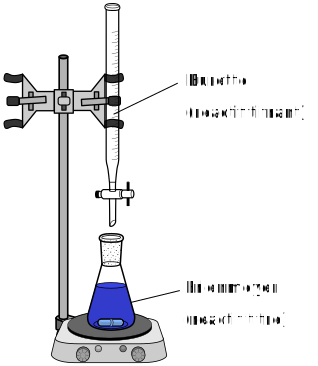
\includegraphics[width=5cm]{images/Acid-base-titration-fr.png}}
	\caption{Titrage acido-basique}
\end{figure}

Simulation sur Dozzaqueux

Possibilité de repérer le virage par pH-métrie ou avec un indicateur coloré.


\section{Oxydants et réducteurs}
\underline{Niveau :} lycée

\underline{Prérequis :} Formules de Lewis , réactions acido-basiques, constante chimique de réaction, sens d'évolution

\underline{Biblio :} Fosset, Dunod PCSI et PC, Cachau, Maréchal

\subsection{Oxydants et réducteurs}
\subsubsection{Caractère oxydant ou réducteur d'une espèce}

\fbox{
\begin{minipage}{0.90\textwidth}
Un réducteur est une espèce (atomique, moléculaire ou ionique) susceptible de céder un ou plusieurs
électrons

Un oxydant est une espèce (atomique, moléculaire ou ionique) susceptible de capter un ou plusieurs
électrons.
\end{minipage}
}

A tout oxydant correspond un réducteur, selon le schéma formel appelé demi-équation d’oxydoréduction
(ou rédox) : $Ox + n e- = Red$

Une réduction correspond à un gain d’électron(s) pour l’élément étudié ;
Une oxydation correspond à une perte d’électron(s) pour l’élément étudié.

\subsubsection{Nombre d'oxydation}

\textit{Manip 1 : Principe d'un éthylotest, Expériences de chimie organique, Blanchard}
\subsection{Transfert électronique et piles}

\subsubsection{Pile Daniell}
\textit{Manip 2 : Pile Daniell}

Voir au-dessus

\subsubsection{Electrode et transferts électronique}

\subsubsection{Potentiel redox et fem de la pile}

ccl : ouverture sur la corrosion
\section{Chimie analytique quantitative et fiabilité}
\underline{Niveau :} lycée

\underline{Prérequis :} Tableau d'avancement, réactif limitant, proportions stoechiométriques, réactions acido-basiques, incertitudes

\underline{Biblio :} Chimie expérimentale Maréchal Dunod, Chimie analytique Masson

Enjeux industriels, sanitaires, alimentaires, médicaments

\underline{définition dosage :} méthode visant à déterminer précisémment la concentration d'une espèce chimique en solution

\subsection{Dosage par étalonnage conductimétrique}
\subsubsection{Principe : loi de Kohlrausch}
\subsubsection{Mise en oeuvre expérimentale}
\textit{Manip 1 : Dosage par étalonnage du sérum physiologique : détermination de la concentration en NaCl(aq), Maréchal}
\subsection{Dosage par titrage}
\subsubsection{Titrage colorimétrique}
\textit{Manip 2 : Titrage colorimétrique du vinaigre par la soude, La Chimie Expérimentale : chimie générale, J.F. Le Maréchal, Dunod, 1999 (p19-20)}
\subsubsection{Equivalence}
\subsubsection{Titrage conductimétrique}
simulation sur Dozzaqueux, avec la même équation
\section{Evolution spontanée d'un système chimique}
\underline{Niveau :} lycée
\underline{Prérequis :} Tableau d’avancement, Loi de Beer-Lambert, Réaction d’oxydo-réduction, Courant électrique, Dosage par étalonnage

\underline{Biblio :}Tout-en-un PCSI, chimie aux éditions Dunod par Bruno Fosset; Tout-en-un PC-PC*, chimie aux éditions Dunod B    runo Fosset; 100 manipulations de chimie analytique Mesplède; Chimie générale Le Maréchal; Chimie PCSI-PC Dunod; livres à programme
    s (Terminale spécialité Nathan/Belin)
 
\subsection{Equilibre et critère d'évolution spontanée}
Spontané : une transformation a une évolution spontanée si le système évolue de l’état initial vers
\subsubsection{Transformation totale ou non totale}
l’état final sans intervention extérieure.

Transformation totale/non totale

\textit{Manip 1 : Réaction d’oxydo-réduction entre Cu2+ et Fe, Le Maréchal p49}
\subsubsection{Quotient de réaction et constante d'équilibre}
Constante d'équilibre :

Quotient de réaction :

Propriétés :
\begin{itemize}
	\item K ne dépend que de la température
	\item K ne dépend pas de la composition initiale du système
\item On considèrera qu’une réaction est totale si la disparition d’un réactif intervient, ou si $K>10^4$
\end{itemize}
Equilibre dynamique :

\textit{Manip 2 : Complexe du fer : Détermination de la constante de formation du complexe Fe(SCN)2+, Mesplède p119 -p 176 (mix des deux)}

\subsubsection{Evolution spontanée d'un système chimique}

Après avoir défini ces grandeurs mathématiques, ce qui nous intéresse réellement c’est de savoir
comment vont évoluer nos systèmes chimiques. On a pour cela le critère d’évolution spontanée :

Tout système chimique, hors équilibre, évolue spontanément vers un état d’équilibre
Ce principe va permettre de déterminer, à partir de la composition initiale, dans quel sens la réaction
va se produire

On va dans un premier temps définir le sens direct et le sens indirect d’une équation (le faire sur
notre exemple)

• Si Qi=K, alors il n’y a pas d’évolution, car le système est à l’équilibre

• Si Qi<K, alors le système évolue dans le sens direct. Les réactifs se consomment peu à peu
et les produits se forment. Q va alors augmenter jusqu’à atteindre K

• Si Qi>K, alors le système évolue dans le sens indirect, le quotient de réaction va diminuer
jusqu’à atteindre K

\subsection{Transfert spontané d'électron et oxydo-réduction}
\subsubsection{Transfert direct et indirect d'électrons}
couple redox en jeu, demi-équations

\[Fe^{2+}(aq) + Cu(s) \rightarrow Fe(s) +Cu^{2+}(aq)\]

Ppe d'une pile

\subsubsection{Constitution d'une pile}
\textit{Manip 3 : pile Daniell}
Une pile est constituée de deux demi-piles reliées par un fil et un pont salin. Chaque demi-pile
contient les espèces conjuguées d’un même couple oxydant-réducteur : faire un schéma
Le circuit est fermé grâce aux fils électriques et grâce au pont salin : en effet, celui-ci est composé
souvent d’ions qui se déplacent pour assurer la fermeture du circuit électrique et pour assurer la
neutralité de chacune des demi-piles.
Si les couples sont constitués d’un métal solide, cela constitue l’électrode qui va permettre le
passage des électrons dans le circuit électrique. Sinon, on utilisera une électrode de platine.
On va s’intéresser à une pile particulière Cuivre/Fer.

\[Fe^{2+}(aq) + 2e^{-} = Fe(s)\]

\[Cu(s) = Cu^{2+} + 2e^{-}\]

• Détermination de la polarité d’une pile : déterminer la tension à vide de la pile, c’est-à-dire
lorsqu’elle ne débite pas encore de courant (on en déduit que la borne négative est celle du
fer).

• Anode = borne -, siège de l’oxydation : libération d’électrons
Cathode= borne +, siège de la réduction : consommation d’électrons

• On peut également observer un courant qui passe si on branche la pile et si on place un
ampèremètre en série avec une résistance : en effet, objectif en de la pile : transformer de
l’énergie chimique en énergie électrique et pouvoir la récupérer grâce au circuit extérieur.

\subsubsection{Fonctionnement d'une pile}
Au cours du fonctionnement de la pile, le système évolue vers l’équilibre, et donc le quotient de
réaction évolue pour atteindre la constante d’équilibre. A l’équilibre, la pile ne va plus fonctionner :
elle est dite usée. On va essayer de quantifier son fonctionnement à l’aide de la grandeur capacité,
qu’on note C.
Def capacité : c’est la quantité d’électricité maximale que l’on peut faire circuler dans la pile
jusqu’à ce qu’elle soit à l’équilibre chimique
quantité de matière d’électrons échangée au cours de la vie

\[Q=i\Delta T= n(e^{-})e N_a\]
de la pile. La quantité maximale d’électrons échangée se détermine à partir de la quantité du réactif
limitant (application à la réaction considérée)

\section{Cinétique et catalyse}
\underline{Niveau :} lycée

\underline{Prérequis :} notion d'avancement, réaction d'oxydo-réduction, spectrophotométrie

\underline{Biblio :} Dunod PCSI, livre à pgrm (Hachette TS), Mesplède 

\subsection{Durée d'une réaction et facteurs cinétiques}
\subsubsection{Réaction lente et réaction rapide}
critère visible à l'oeil nu ($t>0.1$)

définitions : durée d’une réaction (l’avancement atteint sa valeur maximal, le système est à
l’équilibre)

Notion introduite par deux petites manipulations (exp 1 et 2)
\subsubsection{Facteurs cinétiques}

Paramètres influant sur la cinétique :
Température, concentration, surface de contact, Concentration en réactifs

illustré par des simulations et une petite manip (exp 3)
\subsection{Suivi cinétique}

définitions

suivi cinétique : suivi expérimental de l’évolution d’une concentration en réactif ou en produit
au cours d’une réaction.

méthode chimiques (prélèvements du milieu réactionnel, trempe chimique et titrage)

méthode physique (suivre une grandeur physique reliée simplement aux concentrations comme
l’absorbance, la conductimétrie, la pression)=> plus pratique

détails spectrophotométrie, dessin spectre, allure de la courbe A(t) attendue

loi de Beer-Lambert $A=l \epsilon c$ car une seule espèce coloré

définition : temps de demi-réaction (temps auquel l’avancement est la moitié de l’avancement
maximal)

\subsubsection{Principe}
définition, ppe


\subsubsection{Par spectophotométrie}
\textit{Manip 4 :}
\subsection{Catalyse}
\subsubsection{Définition}
Un catalyseur est une espèce capable d’accélérer une réaction. Le catalyseur n’apparaît pas dans
le bilan de la réaction.
\subsubsection{Types de catalyse}
homogène, hétérogène, enzymatique (avantages et inconvénients)

Homogène ; le catalyseur est dans la même phase que les réactifs
Hétérogène : le catalyseur est dans une phase différente
Enzymatique : le catalyseur est une enzyme
illustré par une manip (exp 5)
tableau : Avantages/inconvénients pour chacune
Homogène
Hétérogène
Enzymatique
Avantages Facile et efficace Catalyseur facile à
récupérer
Inconvénients Catalyseur difficile àrécupérer Chère (métaux nobles) Sélective
Conclusion : exemples et applications
Le sucre dans le café
Conservation des aliments
Autocuiseur
Photosynthèse et mûrissement (catalyse par des photons)
Transformation (lente) des diamants en graphite à l’échelle géologique
Pot d’échappement catalytique
Peu chère, écologique,
sélective
\underline{ccl :} exemples et applications

\section{Synthèse chimique : aspect macroscopique et mécanisme réactionnel}
\underline{Niveau :} lycée

\underline{Prérequis :} Groupe caractéristique et fonction, polarisibilité et polarisation, titrage acido-basique, CCM

\textit{Manip 1 : Synthèse du nylon}

Manip introductive
\subsection{Aspects macroscopiques}
\subsubsection{Modification de groupe}
\subsubsection{Grandes catégories de réactions}
\subsubsection{Mise en oeuvre et aspects cinétiques}

\textit{Manip 2 : Saponification du benzoate d’éthyle caractérisation au banc Köfler et CCM}

CCM avec 30\% cyclohexane et 70\% éthanoate d'éthyle

conditions différente (avec et sans chauffage, avec et sans catalyse) et titrage colorimétrique avec BBT 

déf catalyseur
\subsection{Modélisation microscopique}
\subsubsection{Site donneur et site accepteur}
\subsubsection{Mécanisme réactionnel}
déf

exemple estérification de Fisher

déf intermédiaire réactionnel

\subsection{Interprétation microscopique de l'influence des facteurs cinétiques}
\subsubsection{Ajout de catalyseur}
animation edumedia
\subsubsection{Influence de la température}

ccl : intérêt du montage à reflux
\section{Séparations, purifications et contrôles de pureté}
\underline{Niveau :} lycée

\underline{Prérequis :} avancement, rendement, densité, température de fusion, solubilité, CCM, acides et bases

\underline{Biblio :} Daumarie, Chimie organique expérimentale, M.Blanchard, Techniques expérimentales en chimie, Bernard \& al. : fiches sur les différentes techniques 

\textit{Manip : Synthèse de Cannizzaro puis séparations identification et purifications, Chimie organique expérimentale, M.Blanchard}
\subsection{Séparations}
\subsubsection{Séparation liquide-liquide}
Décantation
\subsubsection{Séparation liquide-solide}
Filtration
\subsection{Identification et contrôle de pureté}
\subsubsection{CCM}
essai dichlore, puis des solvants plus protiques (acétone\dots)
\subsubsection{Température de fusion}
banc Köffler
\subsubsection{Autres méthodes}
indice de réfraction, 
\subsection{Purification}
\subsubsection{Purification des solides}
Recristallisation dans un minimum de solvant
\subsubsection{Purification des liquides}
Distillation fractionnée
\section{Distillation et diagrammes binaires}
\underline{Niveau :} lycée

\underline{Prérequis :} corps purs et changements d'états

\underline{Biblio :} Chimie tout-en-un PC-PC* Fosset Dunod

\subsection{Mélanges binaires}
\subsubsection{Définition}
\underline{Mélange binaire :} solution composée de deux corps purs

\textit{Manip 1 : Example de mélanges homogènes (eau+sirop) et hétérogène (eau+huile d'olive)} 
\subsubsection{Analyse thermique}
\textbf{Cas de l'eau pure}
\textit{Manip 2 : Courbe d'analyse thermique de l'eau pure et d'un mélange eau-éthanol à 50/50}

Chauffage à flux constant, enregistrement avec un thermocouple

\textbf{Cas d'un mélange binaire homogène}
\subsection{Diagramme binaire isobare}
\subsubsection{Fraction molaire et fractions massique}
définition

mélange binaire caractérisé par sa composition

\subsubsection{Construction du diagramme}
à partir des courbes d'analyse thermique
\subsubsection{Utilisation du diagramme}
théorème de l'horizontale

cas d'un azéotrope

\subsection{Application à la distillation}
\subsubsection{Distillation simple}
\subsubsection{Distillation fractionnée}
Même montage mais avec une colonne de Vigreux

\textit{Manip 3 : Distillation fractionnée d'un mélange eau-éthanol à 10\% et caractérisation avec la masse volumique}
\section{Caractérisation par spectroscopie en synthèse organique}

\underline{Niveau :} lycée

\underline{Prérequis :} formule topologique, nomenclature, absorbance et loi de Beer-Lambert, liaisons hydrogènes, réactions acides-bases

\underline{Biblio :} Livres à programmes (Nathan et Belin) 
\subsection{Spectroscopie UV-visible}
\subsection{Spectroscopie infrarouge}
\subsection{Spectroscopie RMN}
\section{Stratégie de synthèse}
\underline{Niveau :} lycée

\underline{Prérequis :}

\underline{Biblio :} Livres à programme (Hatier TS 2020, Nathan TS 2020, Bordas TS 2020), Chimie3, culuturesciencechimie

\subsection{Choix du protocole}
risques, coût et qualité des réactifs
montage à reflux : chauffer (cinétique) sans perdre les vapeurs
\subsection{Optimisation de la vitesse de formation des produits}
manip avec ou sans chauffage, avec ou sans catalyse puis trempe et titrage
formation d'un ester (ethanoate d'ethyle) à partir de l'éthanol et de l'acide éthanoïque, catalyse acide 
catalyse et chauffage accélèrent la réaction
\subsection{Optimisation de la quantité de produit formé}
rendement
réactif en excès ou éliminer un produit (Dean-Stark) pour déplacer l'équilibre
Puis identifier et  purifier pduit
\subsection{Optimisation de la sélectivité}
\subsubsection{Synthèse sélective}
synthèse paracétamol, réactifs chimiosélectifs
\subsubsection{Protection et déprotection de groupes fonctionnels}
acide aminé, séquence protection réaction déprotection
\section{Molécules d'interêt biologique}
\underline{Niveau :} lycée

\underline{Prérequis :} Enantiomérie, CCM, température de fusion, électrolyse, oxydo-réduction

\underline{Biblio :} 
\subsection{Molécules du vivant}
\textit{Manip 1 : Extraction du limonène des écorces d'orange CCM et pouvoir rotatoire}

colorant, arôme et chiralité

ex thalidomide
\subsection{Molécule de synthèse : médicament}

\textit{Manip 2 : Synthèse du paracétamol et caractérisation par CCM/Köffler}

\subsection{Produit désinfectant}

\textit{Manip 3 : Synthèse et titrage d'une eau de Javel, Cachau}

\underline{Ccl :} nombreuses molécules appli médicales/alimentaires

\section{Solvants}
\underline{Niveau :} CPGE 

\underline{Prérequis :} interactions intermoléculaires (Van der Waals et liaison H), conductimétrie, dosages, cinétique

\underline{Biblio :} Daumarie, Dunod , culturesciencechimie pour les solvants et chimie verte

\textit{Manip 1 : Dissolution de sel dans eau et cyclohexane (qualitative rapide)}
\subsection{Caractéristiques des solvants et dissolution}
\subsubsection{Moment dipolaire et ionisation}
\subsubsection{Permittivité relative et dissociation}
\subsubsection{Solvatation et proticité}
\textit{Manip 2 : Dissolution I2 dans deux tubes à essai : eau et cyclohexane (qualitative rapide)}
\subsubsection{Catégories de solvants}
\subsection{Miscibilité et solubilité}
\subsubsection{Miscibilité}
\textit{Manip 3 : Miscibilité eau/éthanol/cyclohexane (qualitative rapide)}
\subsubsection{Coefficient de partage}
\textit{Manip 4 : Détermination du coefficient de partage du diode entre l’eau et le cyclohexane}
\subsection{Applications : Extraction liquide-liquide}
Choix du solvant

\textit{Manip 5 : Cannizzaro extraction liquide-liquide, Blanchard}
\section{Classification périodique}
\underline{Niveau :} CPGE 

\underline{Prérequis :}

\underline{Biblio :} 
\subsection{Construction du tableau}
\subsubsection{Histoire}
\subsubsection{Classification actuelle}
\subsection{Lien avec la structure électronique}
\subsection{Propriétés atomiques}
\subsubsection{Energie d'ionisation et affinité électronique}
\subsubsection{Electronégativité}
\subsubsection{Rayon atomique}
\subsection{Propriétés physiques et chimiques}
\subsubsection{Réduction}
\subsubsection{Oxydation}
\section{Solides cristallins}
\underline{Niveau :} CPGE 

\underline{Prérequis :} Types et énergies de liaisons, diffraction par un réseau

\underline{Biblio :} Dunod tout-en-un, Masson intro à la physique du solide, Dunac et Maréchal

\subsection{Des observations au modèle}

\subsubsection{Observations}
\subsubsection{Définition}
\subsubsection{Modèle du cristal parfait}

\subsection{Différents types de cristaux}
\subsubsection{Energie de liaison}
\subsubsection{Taille de liaison}

\subsection{Compacité}
\subsubsection{Modèle des sphères dures}
\subsubsection{Coordinence et compacité}
\subsubsection{Formes allotropes}
\section{Corps purs et mélanges binaires}
\underline{Niveau :} CPGE (PSI)

\underline{Prérequis :} premier principe, potentiels et identités thermodynamiques

\underline{Biblio :} Dunod Tout en un PSI, Daumarie
\subsection{Changement d'état du corps pur}
\subsubsection{Equilibre pour un corps pur diphasés}
potentiel chimique, enthalpie libre
\subsubsection{Variance d'un système}
définition variance
définition température de changement d'état 
\subsubsection{Courbe d'analyse thermique}
palier
\subsection{Changement d'état d'un mélange miscible}
\subsubsection{Courbe d'analyse thermique}
rupture de pente
\subsubsection{Diagramme binaire isobare d'un mélange idéal}
construction à partir des courbes
\subsubsection{Exploitation des diagrammes}
théorème de l'horizontale et des moments.
\subsubsection{Mélange non idéal}

\subsection{Changement d'état d'un mélange non miscible}
\subsubsection{Courbe d'analyse thermique}
\subsubsection{Diagramme binaire isobare}

\underline{ccl :} étude des alliages, salage des routes, surfusion
construction à partir des courbes
\section{Application du premier principe de la thermodynamique à la réaction chimique}
\underline{Niveau :} CPGE 

\underline{Prérequis :} premier principe, calorimétrie

\underline{Biblio :} 

\textit{Manip 1 : Dissolution d'urée dans l'eau mesure du refroidissement au thermomètre}
\subsection{Fonctions d'état}
\subsubsection{Premier principe}
énoncé : sys fermé

déf : monochore/isochore, monobare

ppe bombe calorimétrique
\subsubsection{Paramètres d'état d'interêt}
\subsection{Utilisation et convention}
\subsubsection{En pratique}
\subsubsection{Convention et état standard de référence}
déf ESR

déf enthalpie standard de formation
\subsection{Approximation d'Ellingham et conséquences}
énoncé

\textit{Manip 3 : mesure de l’enthalpie d’hydratation de Na 2 (CO 3 ) au calorimètre}
\section{Détermination de constantes d'équilibre}
\underline{Niveau :} CPGE 

\underline{Prérequis :} solubilité, équilibre chimique

\underline{Biblio :} Dunod PCSI, Cachau redox, Cachau acide-base, Daumarie

Intro :

\textit{Manip 1 : Comparaison de la force de différentes bases, Cachau Acide-Base p. 108}

\subsection{Détermination de constantes d'équilibre en solution : l'iode}
\subsubsection{Coefficient de partage du diiode}
\textit{Manip 2 : Determination du coefficient de partage de I2, Florilege d’expérience de chimie, Daumarie, p. 125}
\subsubsection{Constante de formation du complexe I 3-}
\subsubsection{Constante de solubilité de l'iodure de plomb}
\subsection{Détermination de constantes d'équilibre électrochimique : la pile Fer-Iode}
\textit{Manip 3 : Pile Fer-Iode, Florilege d’expérience de chimie, p. 257}
\subsubsection{Potentiels standard des couples Ox/Red en jeu}
\subsubsection{Force électromotrice de la pile et constante d'équilibre d'oxydo-réduction}
\subsubsection{Dépendance en température de la fem}
exp pluie d'or ?

\section{Cinétique homogène}
\underline{Niveau :} CPGE 

\underline{Prérequis :} Avancement, Oxydo-réduction, Temps de demi-réaction, Loi de Beer-Lambert

\underline{Biblio :} Mesplède

Définitions : cinétique chimique
homogène

\subsection{Cinétique d'une réaction chimique}
\subsubsection{Vitesse de réaction}
réaction lente et rapide

\textit{Manip 1 : précipitation de AgI}

Ag+(aq) + I-(aq) = AgI(s)
Rapide

\textit{Manip 2 :Oxydation des ions iodure par les ions peroxodisulfate}

2 I-(aq) +S208 2-(aq) =I2(aq) +2 S2O4 2-

\subsubsection{Méthode de mesure, suivi cinétique}
\textit{Manip 3 : Oxydation des ions iodures par le peroxodisulfate, suivi par spectrophotométrie, Mesplède}
\subsection{Influence de la concentration}
\subsubsection{Notion d'ordre}
\subsubsection{Lois de vitesse}
\subsubsection{Déterminer un ordre}
\subsection{Influence de la température}
\subsubsection{Loi d'Arrhénius}

\section{Evolution et équilibre chimique}
\underline{Niveau :} CPGE 

\underline{Prérequis :} premier et second principe de la thermodynamique, potentiel chimique, avancement, acide-base

\underline{Biblio :} Dunod Tout en un PC, Cachau acide-base

\textit{Manip 1 : Déplacement de l’équilibre NO 2 =N 2 O 4 par variation de la température et de la pression, BUP n°879 (1)}
\subsection{Caractérisation de l’équilibre}
\subsubsection{Evolution du système}
enthalpie libre G
\subsubsection{Constante d’équilibre}
\textit{Manip 2 : Détermination du pKA de l’acide éthanoique par dosage de l’acide éthanoïque par la soude, Cachau}
\subsection{Déplacement d’équilibre}
\subsubsection{Variance}
\subsubsection{Influence de la température}
loi de Van’t Hoff
\subsubsection{Influence de la pression}
Loi de Le Chatelier

retour sur la manip 1
\section{Diagramme potentiel-pH (construction exclue)}
\underline{Niveau :} CPGE 

\underline{Prérequis :} réactions d'oxydo-réduction, acido-basiques, titrages, construction d'un diagramme potentiel-pH

\underline{Biblio :} Cachau, Sarrazin, Maréchal

\subsection{Réactivité}
\textit{Manip 1 : Couples Fe (III)/Fe(II) et I2/I-, l'Oxydoréduction Sarrazin p 126}

Superposer les diagrammes du fer et de l'iode avec chimigéné
\subsection{Stabilité}
\textit{Manip 2 : Dismutation de l'iode en milieu basique, l'Oxydoréduction Sarrazin p 128}
\subsection{Application : dosage de Winkler}
\textit{Manip 3 : Dosage de Winkler, La chimie expérimentale, Le Maréchal p 78}
\section{Optimisation d'un procédé chimique}
\underline{Niveau :} CPGE 

\underline{Prérequis :} premier et second principe, cinétique chimique, critère d'évolution spontané

\underline{Biblio :} 

intro : exemple du procédé Haber-Bosch

\subsection{Notion de variance}
\subsubsection{Variance}
\subsubsection{Déplacement et rupture d'équilibre}
\subsection{Optimisation thermodynamique}
lois de modérations
\subsubsection{Influence de la pression}
Loi de le Châtelier
\textit{Manip 1 : Equilibre entre le tétra oxyde de diazote et le dioxyde d’azote, BUP n°879 décembre 2005, page 1173-1179 \url{http://bupdoc.udppc.asso.fr/consultation/article-bup.php?ID\_fiche=19222}}
\subsubsection{Influence de la température}
Loi de Van't hoff
\textit{Manip 2 : Echange de ligand, Experience de chimie pour le capes page 70}
\subsection{Optimisation cinétique}
\subsubsection{Energie d'activation}
\textit{Manip 3: Experience du coucher de soleil, dismutation des ions thiosulfates, Mesplède : 100 expériences de chimie (générale et analytique) Manipulation 75 p194}
\subsubsection{Catalyse}
\section{Corrosion humide des métaux}
\underline{Niveau :} CPGE 

\underline{Prérequis :} diagrammes de Pourbaix, électronégativité

\underline{Biblio :} Cachau, Dunod PSI, Oxydoréduction Sarrazin

\subsection{Corrosion uniforme}
\subsubsection{Corrosion acide}
\textit{Manip 1 : Mesure du courant de corrosion, L'oxydoréduction Sarrazin p 294}

Montage à 3 électrodes
\subsubsection{Corrosion neutre aérée}
\subsection{Corrosion différentielle}
\textit{Manip 2 : Corrosion différentielle, Cachau redox p 166}
\subsubsection{Corrosion galvanique}
Anode sacrificielle
\subsubsection{Aération différentielle}
Goutte d'Evans

\textit{Manip 3 : Goutte d'Evans, Cachau redox p 167}
\subsubsection{Electrozingage}

\textit{Manip 4 : Electrozingage, Cachau redox p 167 et 278}

\section{Conversion réciproque d'énergie électrique en énergie chimique}
\underline{Niveau :} CPGE 

\underline{Prérequis :} Principes thermo, réaction redox, relation de Nernst, diagrammes potentiel-pH

\underline{Biblio :} BUP 902 electrolyse de l'eau, Cachau redox

\subsection{Conversion d'énergie chimique en énergie électrique : la pile Daniell}
\subsubsection{Etude thermodynamique}
enthalpie de réaction, déterminer expérimentalement celle de la pile Daniell
\textit{Manip 1 : Etude de la pile Daniell, Cachau}
lien avec la fem et l'enthalpie de réaction
\subsubsection{Etude cinétique}
tracé de la courbe courant-potentiel, sys rapide
\subsection{Conversion d'énergie électrique en énergie chimique : électrolyse}
\subsubsection{Efficacité de la synthèse}
\subsubsection{Rendue possible par un blocage cinétique}
ex sys lent avec O2, blocage cinétique
\textit{Manip 2 : Synthèse et titrage de l'eau de Javel}
\section{Solubilité}
\underline{Niveau :} CPGE 

\underline{Prérequis :} équilibre et cte d'équilibre, quotient de réaction, loi de Van t hoff, conductimétrie 

\underline{Biblio :} Dunod PTSI et MPSI

\subsection{Concentration limite et produit de solubilité}
Expérience qualitative
\subsection{Détermination expérimentale}

\textit{Manip : Détermination du pKs de AgCl par potentiométrie (Fosset)}
\subsection{Facteurs influançant la solubilité}
température, ions communs
\textit{Manip : Effet d’ions commun AgCl (Mesplède)}
%\textit{Manip : Influence de la température sur la dissolution de l’acide benzoïque (Fosset)}
pb cinétique

\section{Cinétique électrochimique}
\underline{Niveau :} CPGE 

\underline{Prérequis :} Diagrammes potentiel-pH, oxydo-réduction

\underline{Biblio :} Cachau, Grécias chimie PC, Dunod Fosset Chimie MP, Techniques expérimentales en chimie Bernard Dunod
\textit{Manip 1 : Clou de fer dans l'acide sulfurique, Des expériences de la famille redox Cachau p 256}

Manip introductive, blocage cinétique/couple lent + rôle de l'électrode
\subsection{Vitesse électrochimique}
\subsubsection{Vitesse et intensité}
\subsubsection{Intensité et potentiel}
\textit{Manip 2 : tracé des courbes courant potentiel du fer, Des expériences de la famille redox Cachau p 173}

Faire le montage à trois électrodes
\subsection{Allure des courbes i-E}

couples lents vs couples rapides
\subsubsection{Transfert de charge}
\subsubsection{Transfert de matière}
\subsection{Applications}
\subsubsection{Oxydation du fer}
\subsubsection{Electrolyse : synthèse de l'eau de  Javel}
\textit{Manip 3 : Synthèse de l'eau de Javel et caractérisation des ions ClO- avec KI}
\end{document}
